\documentclass{llncs}

% Configuration for draft version
%\usepackage[center, width=13.5cm, height=22.5cm]{crop}
\usepackage[enable]{easy-todo}
\usepackage{amsmath, amssymb}
\usepackage{bussproofs}
\usepackage{graphicx}
\usepackage{mathtools}
\usepackage{stmaryrd}


\title{Antichain Algorithms for Alternating Finite Automata}
\author{Kei Shirakizawa, Mizuhito Ogawa}
\institute{
  School of Information Science \\
  Japan Advanced Instutute of Science and Technology, Japan \\
  \email{\( \{ \)kei.shirakizawa, mizuhito\( \} \)@jaist.ac.jp}
}

\begin{document}
\maketitle
 
\begin{abstract}
We propose an alternating finite automaton(AFA) based approach for
automata-theoretic theorem proving technique. The technique reduces
satisfiability/validity checking of a quantified formula to emptiness checking
of the regular language which encodes the model of the formula. In the AFA
setting, propositions symbolically represent the reachable states and their
acceptance follows the truth valuation. Antichain algorithm is a practically
efficient method to prune the reachable states which explosively increase in
number. Instead of constructing all reachable states explicitly, we only keep a
set of propositions pairwise incomparable w.r.t. implication to judge the
language emptiness. We experimented our method on the theory of Presburger
arithmetic.
\end{abstract}

\section{Introduction}

A SAT/validity checking problem of a quantified formula is decidable on
structures such as WS1S and FOL of Presburger Arithmetic. Those decidable
fragments of logics are widely used in various automated decision
procedures \cite{KlaEtAl:Mona}.

The structure enjoys decidability typically because it admits quantifier
elimination. So-called "automatic structures", on the other hand, have another
mechanism of deciding the quantified formulas on them \cite{}, where each element
in the carrier set has a string representation and each predicate has a
dedicated automaton which serves as an interpreter. Moreover the string
representation and automaton construction are devised in a way that the regular
set falls in the interpretation of the predicate. \todo{Relationship btw. the
  formula validity and the emptiness of regular set} We can perform set
operations over the regular sets along with the structure of an input formula so
that the resulting automaton recognizes the set of instances which satisfy the
formula. Hence language emptiness checking of the automaton yields decidable
decision procedure for the SAT/validity checking problem.

\todo{Difficulty of the problem, especially for NFA implementation of the
  regular set} Interpreting an existential quantifier sources nondeterminism to
the automaton while interpreting a negation requires the automaton to be
deterministic. The problem is known to have the non-elementary complexity due to
the determinization procedure which causes state explosion through the subset
construction. For finite automata, each state has a complex structure of nesting
sets and tuples due to the repetitive applications of subset and product
constructions. It also makes the acceptance condition counter-intuitive.

\todo{Existing works handle the problem?}
\todo{more in detail} Antichain WS1S \cite{Fiedor2015,Fiedor2017}
\todo{more in detail} Syntactical approach \cite{Traytel15,TraytelN15}
In the AFA setting, propositions symbolically represent reachable states and
their acceptance follows a truth valuation. The determinization is directly
expressed by a sequence of `or' symbols. Expressed by logical connectives, the
complex structure in DFA is handled in a unified manner. The antichain algorithm
which maintains the equisatisfiability is a practically efficient method to
prune the reachable states. AFA naturally allows the equisatisfiable
transformation similar to the antichain algorithm. For each sub-formula of a
proposition we replace it with another sub-formula in the set if they are ordered
by implication. This operation is conducted at the same time the construction
proceeds. As a result, instead of maintaining reachable states we only keep a
set of propositions pairwise incomparable by implication to judge the language
emptiness.

\todo{What's new in our work?}  To handle formula not limited to prefix normal
form, we extend the antichain algorithm from \cite{Wulf2006} to utilize
implication as the pruning criteria. We list our contributions below.

\begin{itemize}
\item Generalization of the antichain algorithm.
\item Bisimulation up to congruence technique \cite{BonchiP13} as well.
\item \todo{An experiment with a randomly generated Presburger formulas}
\item \todo{A performance improvement of the theorem proving technique}
\end{itemize}

And the results shown in this paper contains the following caveats.
\begin{itemize}
\item Our technique cannot handle WS1S formulas.\todo{examples}
\end{itemize}

The paper is organized as follows; Section 2 introduces preliminary definitions
and notations. Section 3 introduces the definition of the alternating automaton
and closure property and DFA conversion. Section 4 describes the antichain
algorithm. We report on the experience with a prototype implementation of the
algorithm in Section 5, and discuss related work in Section 6. We conclude the
paper in Section 7. Appendix contains the omitted proofs.

\section{Preliminaries}

We use boldface font for vectors. For example, \( \mathbf{a} = (a_1, a_2,
\cdots, a_n) \) and \( \mathbf{a}[i] \) denotes the \( i \)-th element of the
vector \( \mathbf{a} \). We take \( \uplus \) for the disjoint union of sets, \(
\mathcal{P}(A) \) for the powerset of the set \( A \). \( \Sigma \) denotes an
alphabet, a finite set of symbols ranged over by \( a, b, c \), and \( \Sigma^*
\) denotes the set of finite words over \( \Sigma \), ranged over by \( w_1,
w_2, \cdots, w_n \). \( \epsilon \) denotes the empty string. We adopt the
standard convention of the literature \cite{Thomas:1997,tata2007} and assume
familiarity with formal language theory \cite{Kozen:1997}.

A finite automaton(\( \mathit{FA} \)) over an alphabet \( \Sigma \) is a 5-tuple
\( \mathcal{M} = (Q, \Sigma, s, F, \delta) \) consisting of a finite set \( Q \)
of states, disjoint from \( \Sigma \), ranged over by \( q, p, r \) or \( q_1,
\cdots , q_n \), an initial state \( s \in Q \), a set of final states \( F
\subseteq Q \), and a transition relation \( \delta \) on \( Q \times \Sigma
\times Q \). We say the \(\mathit{FA}\) is deterministic if \( \delta \) relates
any pairs in \( Q \times \Sigma \) to some unique state, otherwise
non-deterministic.

\( \mathcal{B} = (\{0, 1\}, \bot, \perp, \neg, \wedge, \vee) \) is a boolean
algebra. Let \( Q = \{ q_0, q_1, ..., q_n \} \) be a set of states and we assume
that states are indexed. Here we also use \( Q \) as a set of propositional
variables and let \( q_i \in Q \) vary through \( \mathcal{B} \). A proposition
consists of constants, variables, and logical connectives. Let \( \mathit{Prop}
\) be a set of propositional formulas ranged over by \( \alpha, \beta, \gamma \)
and propositions are defined as follows: \(\alpha ::= q_i \in Q \mid 0 \mid 1
\mid \neg \alpha \mid \alpha \vee \beta \mid \alpha \wedge \beta\). We denote
subsets of \( \mathit{Prop} \) by \( \Gamma, \Pi, \Omega \). The truth
assignments of the proposition \(\mathcal{B}^Q\) is a set of mappings from each
state to boolean algebra. We use \( u, v, t : Q \rightarrow \mathcal{B} \) to
denote each truth assignment.

Since logical equivalence \( \Leftrightarrow \) is an equivalence relation over
\( \mathit{Prop} \), we can construct a quotient \(
\mathit{Prop}_{/\Leftrightarrow} \). If \( \alpha \) and \( \beta \) are
logically equivalent, then they are identical in \(
\mathit{Prop}_{/\Leftrightarrow} \) and belong to the class \( [\alpha] \). For
instance, a set of propositions \( \{ \bot, \neg q_0 \wedge q_0 \} \) is taken for
just the singleton \( \{ [\bot] \} \). Although \( \mathit{Prop} \), the set of
propositions, is infinite, we only consider the finite representative members \(
[\alpha] \in \mathit{Prop}_{/\Leftrightarrow} \). Thus we have \(
|\mathit{Prop}_{/\Leftrightarrow}| = 2^{2^{|Q|}} \). We implicitly refer to the
quotient \( \mathit{Prop}_{/\Leftrightarrow} \) as simply \( \mathit{Prop} \)
and to \( [\alpha] \) as \( \alpha \) respectively.  It follows that if \(
\alpha \Rightarrow \beta \) and \( \beta \Rightarrow \alpha \) then \( \alpha =
\beta \). Note the relation `\( \Rightarrow \)' is a partial ordering over \(
\mathit{Prop} \).

Under a truth assignment \( u \in \mathcal{B}^Q \), the interpretation \( I_u \)
maps a proposition to the boolean algebra, defined as follows: \( (\rm i) \) \(
I_u(c) = c \), where \( c \) is either \( \bot \) or \( \perp \), \( (\rm ii) \)
\( I_u(q_i) = u(q_i) \), and the interpretation for each logical connective is
defined as usual. We write \( u \models \alpha \) if \( I_u(\alpha) = 1 \) and
we abuse the notation to write \( u \models \{\alpha, \beta, .., \gamma \} \) if
\( u \models \alpha \vee \beta \vee ..\vee \gamma \). Note that \( u \not\models
\varnothing \) for any \( u \). By denoting \( \alpha[\beta/q_i] \), we
substitute all occurrences of \( q_i \) in \( \alpha \) with \( \beta \). \(
\alpha[\beta_i/q_i \ ...\ \beta_j/q_j] \) denotes the simultaneous substitution
of those propositional variables \( q_i, ..., q_j \).

Given \( \mathit{Var} \), a set of first-order variables ranged over by \( x_1,
x_2, \cdots, x_n \) and \( \mathit{Pred} \), a set of predicates ranged over by
\( P, Q, R \), let \( \Phi \) be a set of quantified formulas ranged over by \(
\varphi, \psi, \chi \). As shown below, the formula is either a literal or a
logical combination of \( \mathit{FOL} \)-formulas.
\[
  \varphi ::= P \mid \neg P
  \mid \varphi \vee \psi \mid \varphi \wedge \psi
  \mid \forall x_i .\ \varphi(x_i) \mid \exists x_i .\ \varphi(x_i) 
\]

The \( \mathit{FOL} \)-formula with free variables \( x_1, \cdots, x_n \) is
denoted by \( \varphi(x_1, \cdots, x_n) \). We assume the \( \mathit{FOL}
\)-formula is in negation normal form.

\section{Alternating Finite Automaton(AFA)}

Alternating finite automaton is a generalization of
nondeterminism\cite{Yu1997}. An AFA is equipped with a set of
states, whom we take for a set of propositional variables. In AFA setting,
propositions act as states. Accepting states in NFA are, in turn, propositions
satisfied by a boolean value assignment designated in AFA definition.

\begin{definition}
An alternating finite automaton (AFA) is a 5-tuple \( \mathcal{A} = (Q, s, f,
\Sigma, \delta) \), where \( s \in Q \) is an initial state, \( f \in
\mathcal{B}^Q \) is an accept condition and \( \delta: Q \times \Sigma \times
\mathit{Prop} \) is a transition relation.
\end{definition}

The transition relation \( \delta \) designates a transition to a proposition \(
\alpha \) from a state \( q \) reading an input symbol \( a \), and we write \(
\alpha = \delta(q, a) \) as a shorthand for \( (q, a, \alpha) \in \delta \). In
case a transition has multiple destination propositions, we connect them with
disjunction to have the single destination \( \bigvee \{ \alpha \mid (q, a,
\alpha) \in \delta \} \).

Here we introduce a transition function. The auxiliary function \(
\Delta(\alpha, a) \) performs the simultaneous substitution for each
propositional variable \( q_1, ..., q_n \) in \( \alpha \), \( \Delta(\alpha, a)
:= \alpha[\delta(q_1, a)/q_1 \ ...\ \delta(q_n, a)/q_n] \). Reading each symbol
in a string, \( \hat{ \Delta } \) repetitively substitute the record in \(
\delta \) for the variables: \( (\rm i) \) \( \hat{\Delta}(\alpha, \epsilon) :=
\alpha \) \( (\rm ii) \) \( \hat{\Delta}(\alpha, wa) :=
\Delta(\hat{\Delta}(\alpha, w), a) \).

We write \( \alpha \xrightarrow[]w \beta \) to denote \( \beta =
\hat{\Delta}(\alpha, w) \) and we say a word \( w \) is accepted if \( s
\xrightarrow[]w \alpha \) and \( f \models \alpha \).  The language of \(
\mathit{AFA} \) \( \mathcal{A} \) is defined as \( L(\mathcal{A}) = \{ w \mid
\exists \alpha .\ s \xrightarrow[]w \alpha \wedge f \models \alpha \} \).

\begin{example}
Let AFA \( \mathcal{A} \) have 
states \( \{q_0, q_1, q_2\} \) and whose \( \delta \), \( f \) and \(
s \) be specified below.
\begin{align*}
  \begin{array}{c|cc}
    \delta & a & b \\\hline
    q_0 & q_1 \wedge q_2      & 0              \\
    q_1 & q_2                 & q_1 \wedge q_2 \\
    q_2 & \neg q_1 \wedge q_2 & q_1 \vee \neg q_2
  \end{array}&& f = \begin{smallmatrix}q_0 &\mapsto 0\\q_1 &\mapsto 0\\q_2 &\mapsto 1\end{smallmatrix} && s = q_0
\end{align*}

AFA \( \mathcal{A} \) accepts the string ``\( aa \)''. \(q_0
\xrightarrow[]a q_1 \wedge q_2 \xrightarrow[]a (q_2)
\wedge (\neg q_1 \wedge q_2) \equiv \neg q_1 \wedge q_2 \) and \( f \models \neg
q_1 \wedge q_2 \). Both of ``\(a\)'' and ``\( ab \)'' reach to the identical proposition. \(q_0
\xrightarrow[]a q_1 \wedge q_2 \xrightarrow[]b (q_1 \wedge q_2)
\wedge (q_1 \vee \neg q_2) \equiv q_1 \wedge q_2 \).

\end{example}

\subsection{Construction}

We define construction of AFA along with the structure of a \( \mathit{FOL}
\)-formula \( \varphi \). Given an automatic predicate \( P(x_1, x_2) \), We
define an AFA for a literal \( P \) as \( P = (Q, s, f, \Sigma, \Delta) \). At
this point, we abstract away the ternary relation \( \delta \) in favor of its
functional counterpart \( \Delta \). When combining 2 AFAs \( \mathit{M}_\varphi
\) and \( \mathit{M}_\psi \) along with binary logical connectives, we impose an
assumption on them in left and right hand side that their state sets \(
Q_\varphi \) and \( Q_\psi \) are disjoint and we denote union of them as \(
Q_\varphi \uplus Q_\psi \).  The disjointedness makes sure that union of the 2
valuation functions \( f_\varphi \uplus f_\psi \) is again a well-defined
function and the same applies for \( \delta_\varphi \uplus \delta_\psi \). Note
that except for projection, the input-output relation of \( \delta_{\varphi} \)
remains untouched throughout the construction.

\begin{prooftree}
  \AxiomC{
    \( \mathcal{A}_\varphi = (
    Q_\varphi,
    \Sigma,
    s_\varphi,
    f_\varphi,
    \Delta_\varphi) \)
  }
  \AxiomC{
    \( \mathcal{A}_\psi = (
    Q_\psi,
    \Sigma,
    s_\psi,
    f_\psi,
    \Delta_\psi) \)
  }
  \BinaryInfC{
    \( \mathcal{A}_{\varphi \bigcirc \psi} = (
    Q_\varphi \uplus Q_\psi,
    \Sigma,
    s_\varphi \bigcirc s_\psi,
    f_\varphi \uplus f_\psi,
    \Delta_\varphi \circ \Delta_\psi) \) }
\end{prooftree}

, where \( \bigcirc \) stands for either \( \wedge \) or \( \vee \) and \( \circ
\) is the function composition. Since the application of \( \Delta \) doesn't
change the root symbol, any proposition reachable from \(s_\varphi \wedge s_\psi
\) has \( \wedge \) at its root position. Here we propose \(
L(\mathcal{A}_{\varphi \wedge \psi}) = L(\mathcal{A}_{\varphi}) \cap
L(\mathcal{A}_{\psi}) \) because for any string \( w \in \Sigma^* \), \(
s_\varphi \wedge s_\psi \xrightarrow[]w \varphi' \wedge \psi' \) iff \(
s_\varphi \xrightarrow[]w \varphi' \) and \( s_\psi \xrightarrow[]w \psi' \).

Without loss of generality, we can restrict the domain of \(
\Delta_{\mathcal{A}} \) according to the construction. Suppose \(
\mathcal{A}_{\varphi \wedge \psi} \) is a conjunction of 2 automata \(
\mathcal{A}_{\varphi} \) and \( \mathcal{A}_{\psi} \), then the domain of \(
\Delta_{\varphi \wedge \psi} \) can be restricted to a set of propositions whose
top symbol is \( \wedge \). For arbitrary construction, the following equation
holds.
\begin{align*}
  \Delta_{\varphi \bigcirc \psi}(a, \alpha \bigcirc \beta) &=
  \Delta_\varphi(a, \alpha) \bigcirc \Delta_\psi(a, \beta) \\
  \Delta_{\neg \varphi}(a, \neg \alpha) &= \neg \Delta_\varphi(a, \alpha)
\end{align*}

Quantifiers are represented in terms of the transition function rather than the
tuple structure. Unlike the logical connectives we have seen above, the
quantifiers require us to keep the nested structure. Let \( \mathsf{Q} \) stand
for either \( \forall \) or \( \exists \) and the construction affects none of
the 5-tuple elements.

\[
\Delta_{\forall x_i .\ \varphi}(\mathbf{a}, \alpha) =
\bigwedge\limits_{\mathbf{a}' \in \pi_i(\mathbf{a})} 
\{ \Delta_{\varphi}(\alpha, \mathbf{a}') \}
\quad
\Delta_{\exists x_i .\ \varphi}(\mathbf{a}, \alpha) = 
\bigvee  \limits_{\mathbf{a}' \in \pi_i(\mathbf{a})} 
\{ \Delta_{\varphi}(\alpha, \mathbf{a}') \}
\]

From the induction on the length of strings it follows that
\(L(\mathcal{A}_{\forall x_i .\ \varphi}) = \bigcup\limits_{0 \leq n}\{
\mathbf{w} \in \boldsymbol{\Sigma}^n \mid \text{ for all } w \in \Sigma^n ,
\mathbf{w}[w/i]\in L(\mathcal{A}_{\varphi}) \} \).

\begin{lemma}
Let \(\alpha, \beta \in \mathit{Prop} \). If \( \alpha \Rightarrow \beta \) then for all
\( c \in \Sigma \) \( \Delta(\alpha, c) \Rightarrow \Delta(\beta, c) \).
\end{lemma}

\subsection{Bitencoding, the conversion from DFA to AFA}
\begin{theorem}
[Fella, Jurgensen and Yu] A language \( \mathcal{L} \) is accepted by a DFA with
\( 2^k \) states if and only if it's reversed language \( \mathcal{L}^R \) is
accepted by an AFA with \( k + 1 \) states.
\end{theorem}

\begin{example}
  \begin{figure}
    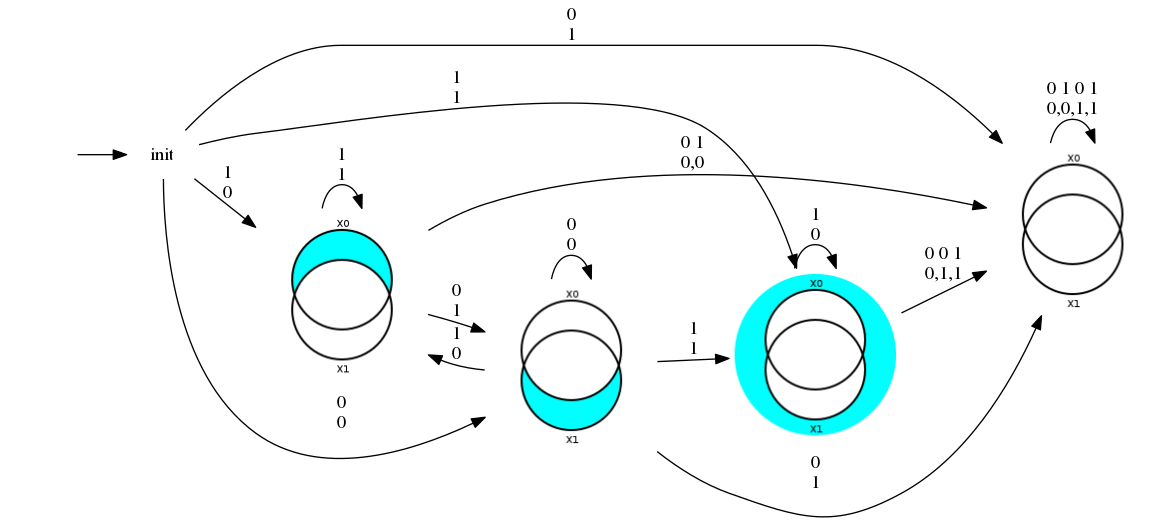
\includegraphics[width=8cm]{images/afa}
  \end{figure}
\end{example}

\section{Algorithm for checking language emptiness}

\begin{example}
  \[ \forall x.\ \forall y.\ -2 x + 3y = 1 \Rightarrow (\exists z.\ x -3z = 1) \wedge (\exists z.\ y -2z = 1) \]

  \paragraph{Linear equation to DFA} By standard method. Figures 1, 2 and 3.
  \paragraph{projection} We perform projection over DFA to express \( \exists \). Fig 2, 3
  \paragraph{cylindrification and product construction}
  We fist perform cylindrification. Cylindrify 2nd character for \( \exists z.\ x -3z = 1
  \) and 1st character for \( \exists z.\ y -2z = 1 \). Secondly we perform
  product construction. Fig 4. By comparing the figures, we can see the language of \(
  -2 x + 3y = 1 \) is contained by that of \( \exists z.\ x -3z = 1 \wedge
  \exists z.\ y -2z = 1 \). Thus implication `\( \Rightarrow \)' holds.

  \begin{figure}
    \label{left}
    \caption{Equation \( -2 x + 3y = 1 \)}
    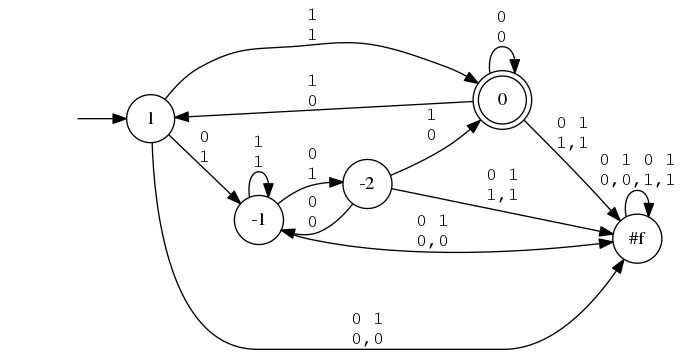
\includegraphics[width=10cm]{images/eq5.png}
  \end{figure}
  \begin{figure}
    \label{rightleft}
    \caption{Equation \( x -3z = 1 \) and \( \exists z.\ x -3z = 1 \)}
    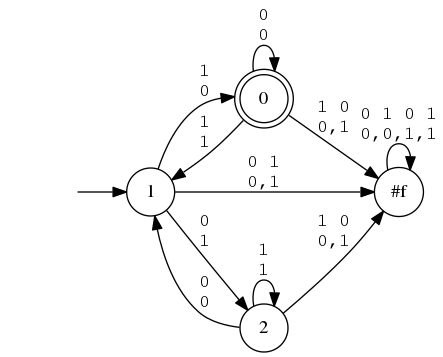
\includegraphics[width=8cm]{images/mod3is1_x.png}
    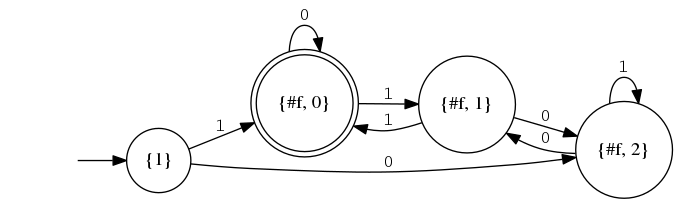
\includegraphics[width=10cm]{images/proj_mod3is1_x.png}
  \end{figure}
  \begin{figure}
    \label{rightright}
    \caption{Equation \( y -2z = 1 \) and \( \exists z.\ y -2z = 1 \)}
    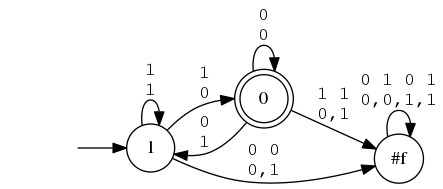
\includegraphics[width=8cm]{images/odd_x.png}
    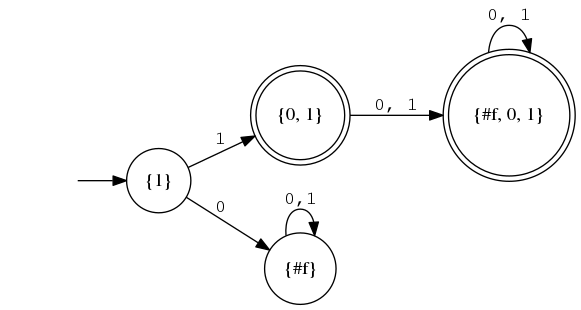
\includegraphics[width=10cm]{images/proj_odd_x.png}
  \end{figure}
  \begin{figure}
    \caption{DFA for \( \exists z.\ x -3z = 1 \wedge \exists z.\ y -2z = 1 \)}
    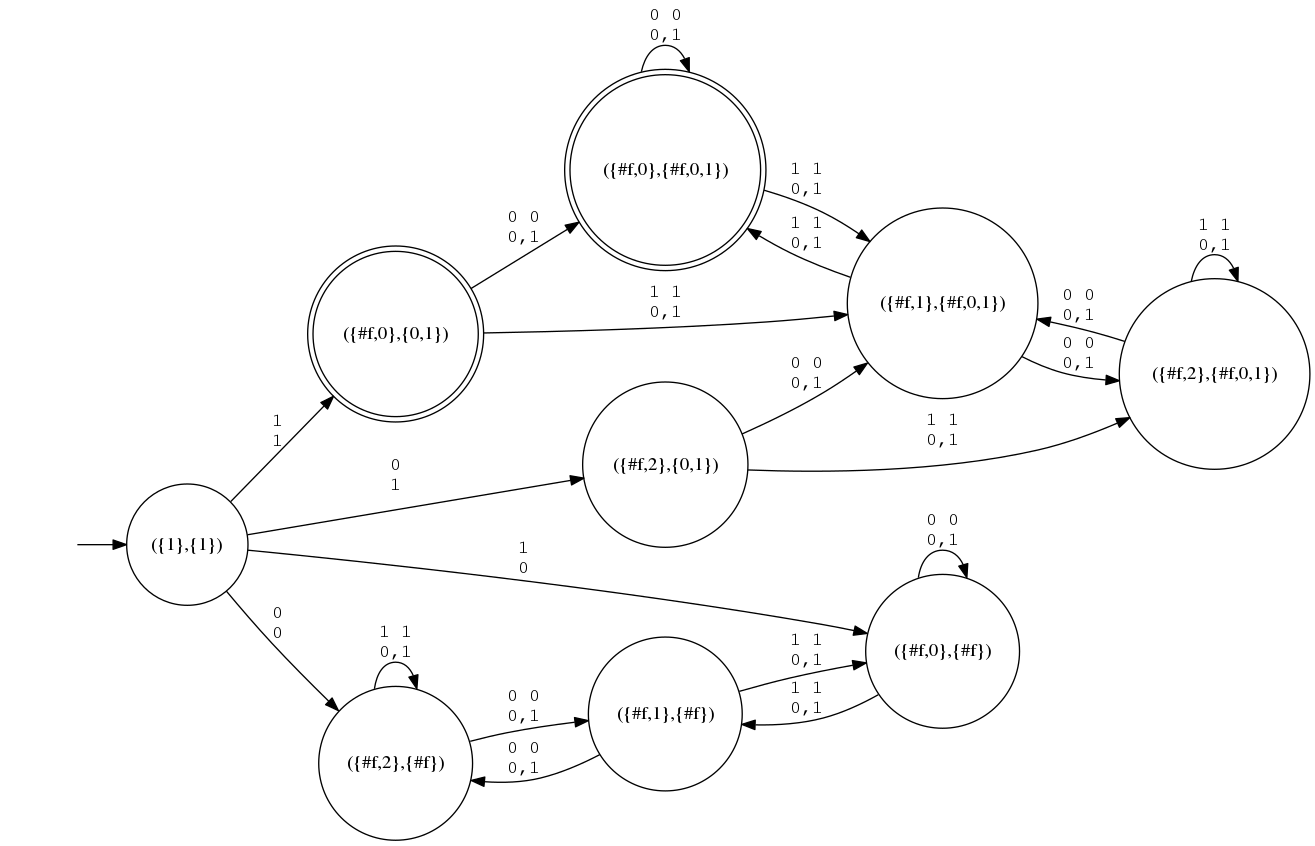
\includegraphics[width=12cm]{images/conjunction.png}
  \end{figure}
  \begin{figure}
    \caption{AFA for \( -2 x + 3y = 1 \)}
    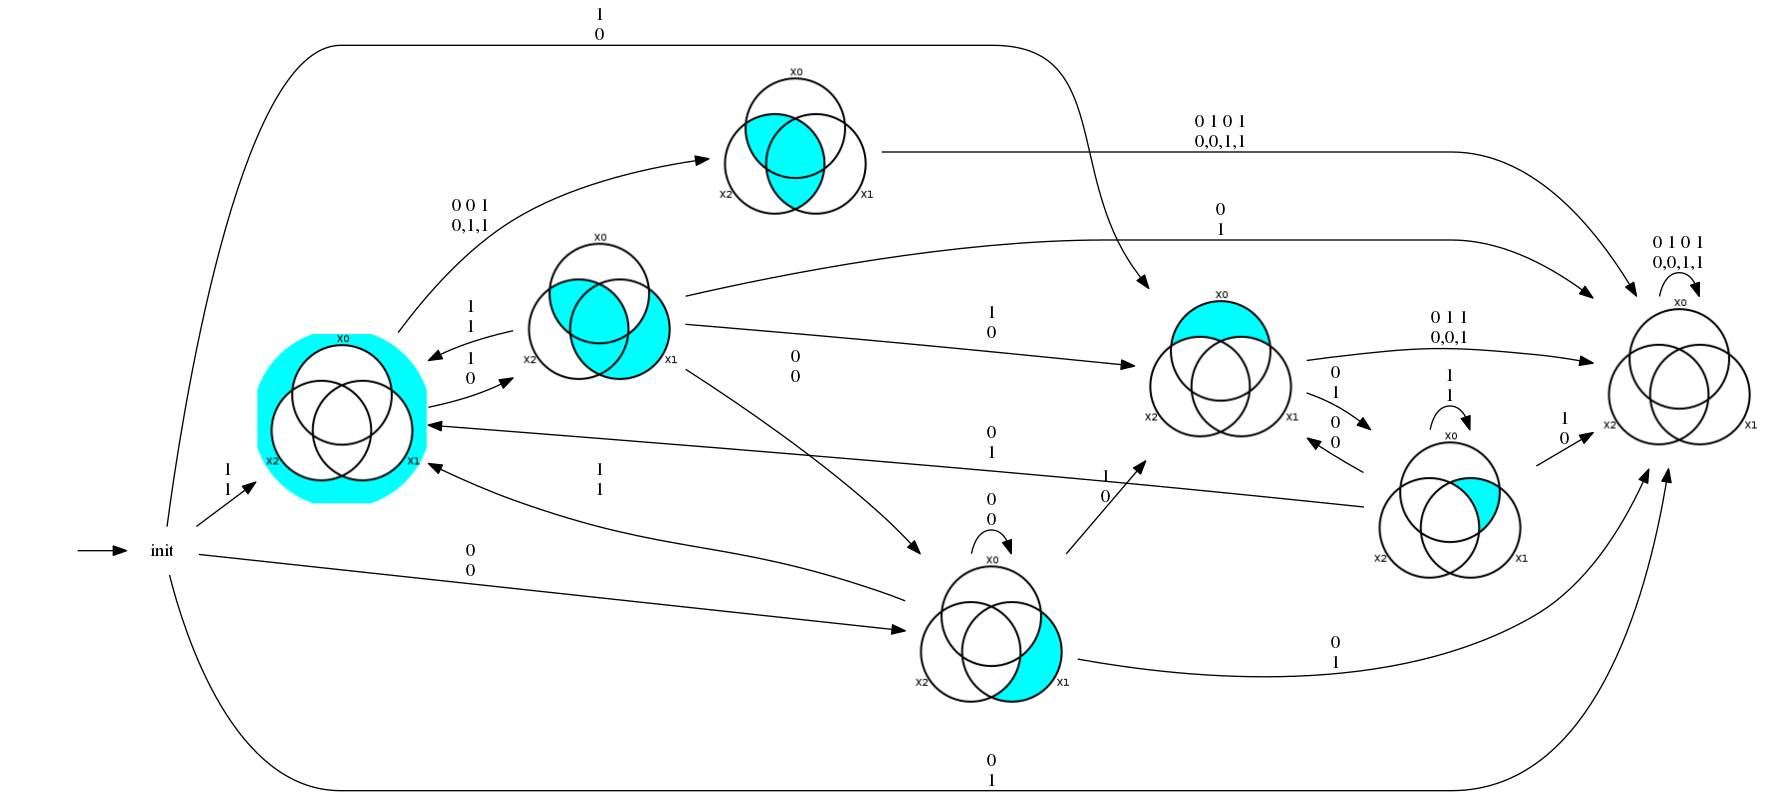
\includegraphics[width=10cm]{images/afa_eq5.png}
  \end{figure}
  \begin{figure}
    \caption{AFA for \( x -3z = 1 \)}
    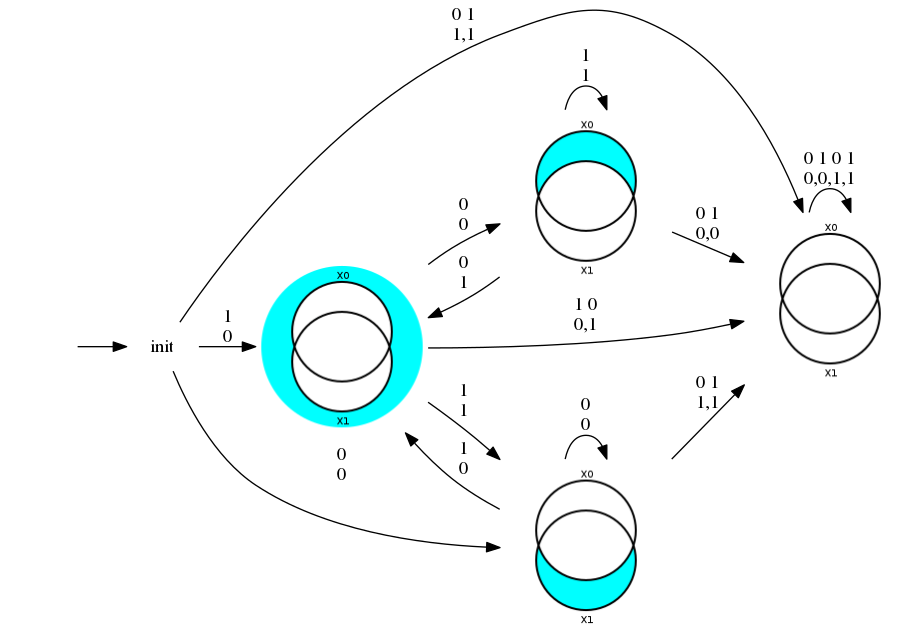
\includegraphics[width=10cm]{images/afa_mod3is1_x.png}
  \end{figure}
  \begin{figure}
    \caption{AFA for \( y -2z = 1 \)}
    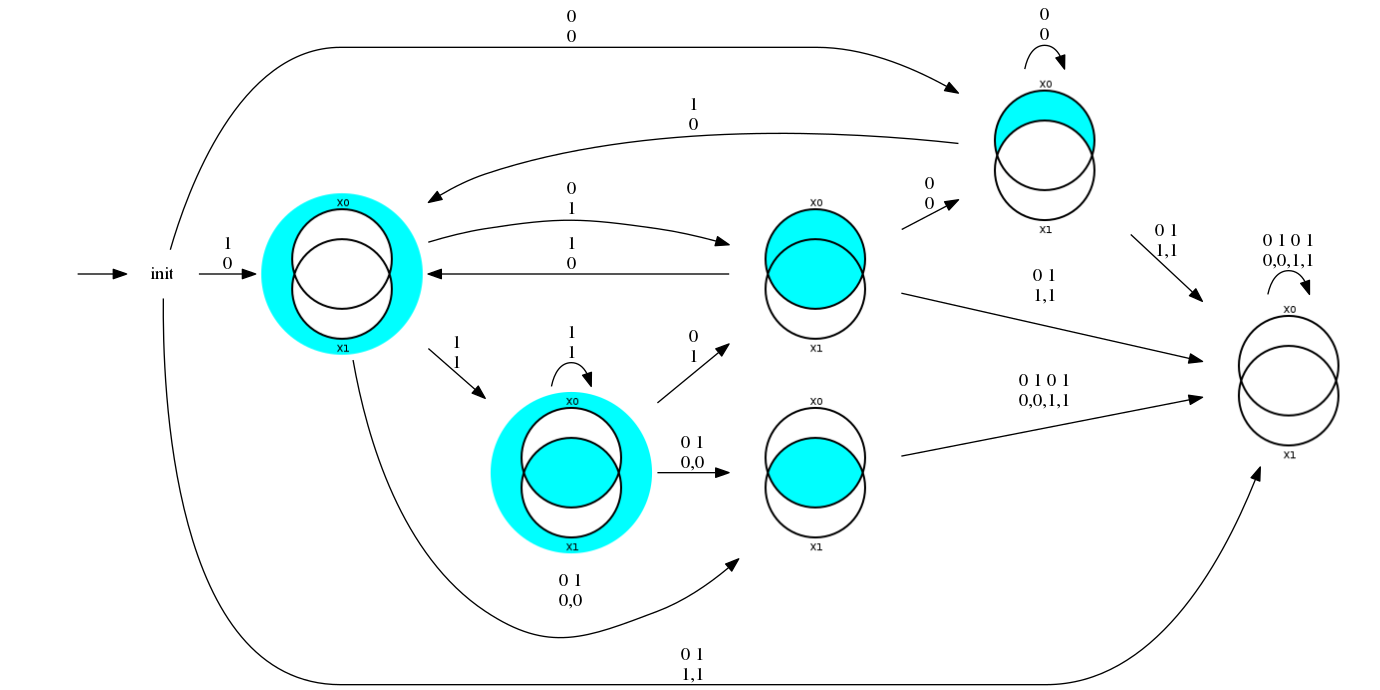
\includegraphics[width=10cm]{images/afa_odd_x.png}
  \end{figure}
\end{example}
\iffalse
Given an \( \mathit{AFA}\) \( \mathcal{A} \), the \textit{emptiness} problem is
to determine \( \mathcal{L}(\mathcal{A}) = \varnothing \).

\begin{definition}
  \begin{align*}
    \mathit{EC}(\Gamma) :=
    \begin{dcases}
    \Gamma \cup \Gamma'              &\text{if } f \models \Gamma \cup \Gamma'
    \\
    \Gamma                           &\text{if } \Gamma \supseteq \Gamma'
    \\
    \mathit{EC}(\Gamma \cup \Gamma') &\text{otherwise } 
    \end{dcases}
    \\
    \text{ where, } \Gamma' :=
    \bigcup\limits_{\alpha \in \Gamma}
    \bigcup\limits_{c \in \Sigma}
    \{ \beta \mid \alpha \xrightarrow[]c \beta \}
    \tag{EC}
  \end{align*}
\end{definition}

\begin{example}
\( \mathit{EC}(\{ q_0 \}) = \{ q_0, 0, q_1 \wedge q_2, \neg q_1 \wedge q_2 \} \).
\end{example}

\begin{definition}
Replace (EC) with (AC) and we have the \( \mathit{antichain} \) algorithm. 
    \begin{align*} \cdots & \text{ where, } \Gamma' :=
    \bigcup\limits_{\alpha \in \Gamma}
    \bigcup\limits_{c \in \Sigma}
    \{
    \beta \mid \alpha \xrightarrow[]c \beta
    \wedge
    \forall \gamma \in \Gamma .\ \beta \not \Rightarrow \gamma
    \}
    \tag{AC}
    \end{align*}
\end{definition}

We say \( \alpha \) and \( \beta \) are congruent if the language beginning from
\( \alpha \) and from \( \beta \) are the same and denote \( \alpha \cong
\beta\).

\begin{definition}
  \begin{align*} \cdots & \text{ where, } \Gamma' :=
    \bigcup\limits_{\alpha \in \Gamma}
    \bigcup\limits_{c \in \Sigma}
    \{
    \beta \mid \alpha \xrightarrow[]c \beta
    \wedge
    \forall \gamma \in \Gamma .\ \beta \not \cong \gamma
    \}
    \tag{CC}
  \end{align*}
\end{definition}

\begin{theorem}
  \begin{itemize}
  \item \(EC(\{s\}) \models \text{ iff }
    \mathcal{L}(\mathcal{A}) \neq \varnothing. \)
  \item \(AC(\{s\}) \models \lceil \text{ iff }
    \mathcal{L}(\mathcal{A}) \neq \varnothing. \)
  \item \(CC(\{s\}) \models \lceil \text{ iff }
    \mathcal{L}(\mathcal{A}) \neq \varnothing. \)
\end{itemize}
\end{theorem}
\fi


\bibliographystyle{splncs04}
\bibliography{reference}
\listoftodos
\end{document}
